% Modelo entidad-relación de la base transaccional spine_oltp.db (sql/oltp.sql).
% Compilar con XeLaTeX: genera er_oltp.pdf (defensa); diagramas.py lo copia a defensa/fig y lo exporta a PNG.
\documentclass[border=6pt]{standalone}
\usepackage{fontspec}
\usepackage[sfdefault]{FiraSans}
\usepackage{tikz}
\usetikzlibrary{positioning, arrows.meta, shapes.multipart, calc, backgrounds}
% Estilo compartido por los diagramas ER y del almacén (colores ITBA, iguales a defensa.tex).
\definecolor{itba}{HTML}{02568A}
\definecolor{itbaclaro}{HTML}{7FA9C8}
\definecolor{itbafondo}{HTML}{EAF1F7}
\definecolor{tinta}{HTML}{1F2933}
\definecolor{gris}{HTML}{8A949E}
\definecolor{alerta}{HTML}{C0392B}
\hyphenpenalty=10000 \exhyphenpenalty=10000   % sin división silábica dentro de las tablas
\tikzset{
  ent/.style={rectangle split, rectangle split parts=2, draw=itba, line width=0.8pt, rounded corners=2pt,
              rectangle split part fill={itba,white}, font=\scriptsize, align=left, inner sep=3pt,
              text width=#1, text=tinta},
  ent/.default=3.4cm,
  hecho/.style={ent=#1, rectangle split part fill={alerta,white}, draw=alerta},
  dimen/.style={ent=#1},
  linea/.style={draw=itba, line width=0.8pt},
  fina/.style={draw=itbaclaro, line width=0.7pt},
  card/.style={font=\footnotesize\bfseries, text=itba, inner sep=1.5pt},
  verbo/.style={font=\scriptsize\itshape, text=tinta, inner sep=1pt},
  nm/.style={draw=alerta, line width=0.8pt, dashed},
  nmtexto/.style={font=\scriptsize\bfseries, text=alerta},
}
\newcommand{\pk}[1]{\textbf{PK}~#1}
\newcommand{\fk}[1]{\textbf{FK}~#1}
\newcommand{\pkfk}[1]{\textbf{PK·FK}~#1}
\newcommand{\nulo}[1]{\textcolor{gris}{\textit{#1}}}
\newcommand{\fkn}[1]{\textbf{FK}~\nulo{#1}}
\newcommand{\llave}[1]{{\upshape\tiny\color{gris}#1}}
% \entidad[ancho]{nombre}{(x,y)}{atributos}
\newcommand{\entidad}[4][3.4cm]{\node[ent=#1] (#2) at #3 {\textcolor{white}{\textbf{\small #2}}\nodepart{two}#4};}
\newcommand{\dimension}[4][3.2cm]{\node[dimen=#1] (#2) at #3 {\textcolor{white}{\textbf{\small #2}}\nodepart{two}#4};}
\newcommand{\hechos}[4][3.6cm]{\node[hecho=#1] (#2) at #3 {\textcolor{white}{\textbf{\small #2}}\nodepart{two}#4};}
% \relacion{inicio}{fin}{verbo}{columna FK}: línea 1 (lado del padre, inicio) —— N (lado del hijo, fin)
\newcommand{\relacion}[4]{%
  \draw[linea] (#1) -- (#2)
    node[pos=0.07, above, card] {1} node[pos=0.93, above, card] {N}
    node[midway, above=1pt, verbo] {#3} node[midway, below=1pt, verbo, align=center] {\llave{#4}};}


\begin{document}
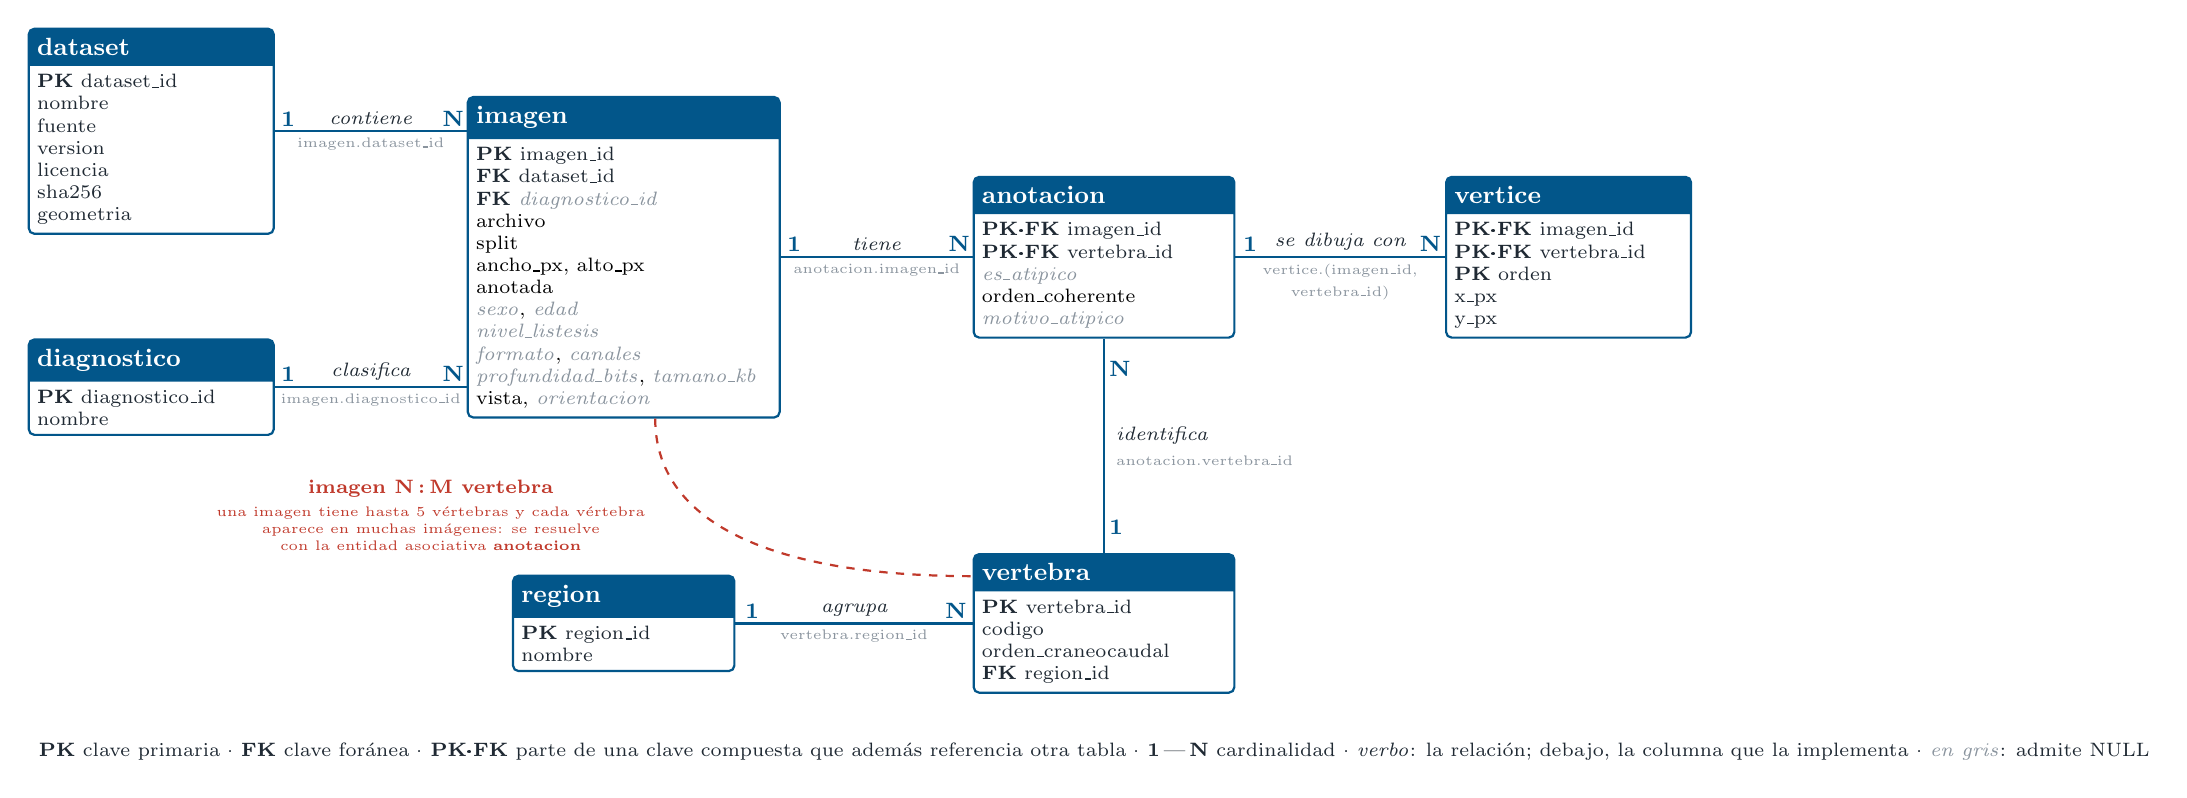
\begin{tikzpicture}
  % ------------------------------------------------------------------ entidades
  \entidad[2.9cm]{dataset}{(0,3.35)}{%
    \pk{dataset\_id}\\nombre\\fuente\\version\\licencia\\sha256\\geometria}
  \entidad[2.9cm]{diagnostico}{(0,0.1)}{\pk{diagnostico\_id}\\nombre}
  \entidad[3.75cm]{imagen}{(6.0,1.75)}{%
    \pk{imagen\_id}\\\fk{dataset\_id}\\\fkn{diagnostico\_id}\\archivo\\split\\ancho\_px, alto\_px\\anotada\\%
    \nulo{sexo}, \nulo{edad}\\\nulo{nivel\_listesis}\\\nulo{formato}, \nulo{canales}\\\nulo{profundidad\_bits}, \nulo{tamano\_kb}\\%
    vista, \nulo{orientacion}}
  \entidad[3.1cm]{anotacion}{(12.1,1.75)}{%
    \pkfk{imagen\_id}\\\pkfk{vertebra\_id}\\\nulo{es\_atipico}\\orden\_coherente\\\nulo{motivo\_atipico}}
  \entidad[2.9cm]{vertice}{(18.0,1.75)}{\pkfk{imagen\_id}\\\pkfk{vertebra\_id}\\\pk{orden}\\x\_px\\y\_px}
  \entidad[3.1cm]{vertebra}{(12.1,-2.9)}{\pk{vertebra\_id}\\codigo\\orden\_craneocaudal\\\fk{region\_id}}
  \entidad[2.6cm]{region}{(6.0,-2.9)}{\pk{region\_id}\\nombre}

  % ------------------------------------------------------------------ relaciones 1:N y llave que la implementa
  \relacion{dataset.east}{dataset.east -| imagen.west}{contiene}{imagen.dataset\_id}
  \relacion{diagnostico.east}{diagnostico.east -| imagen.west}{clasifica}{imagen.diagnostico\_id}
  \relacion{imagen.east}{anotacion.west}{tiene}{anotacion.imagen\_id}
  \relacion{anotacion.east}{vertice.west}{se dibuja con}{\shortstack{vertice.(imagen\_id,\\vertebra\_id)}}
  \relacion{region.east}{vertebra.west}{agrupa}{vertebra.region\_id}
  \draw[linea] (vertebra.north) -- (anotacion.south)
      node[pos=0.12, right, card] {1} node[pos=0.86, right, card] {N}
      node[midway, right=3pt, verbo, align=left] {identifica\\[1pt]\llave{anotacion.vertebra\_id}};

  % ------------------------------------------------------------------ N:M imagen–vértebra
  \draw[nm] ([xshift=0.4cm]imagen.south) .. controls +(0,-1.3) and +(-2.6,0) .. ([yshift=0.6cm]vertebra.west);
  \node[nmtexto, align=center, anchor=north] at (3.55,-0.95) {imagen N\,:\,M vertebra};
  \node[font=\tiny, text=alerta, align=center, anchor=north] at (3.55,-1.3)
      {una imagen tiene hasta 5 vértebras y cada vértebra\\aparece en muchas imágenes: se resuelve\\con la entidad asociativa \textbf{anotacion}};

  % ------------------------------------------------------------------ leyenda
  \node[anchor=north west, font=\scriptsize, text=tinta, align=left] at (-1.55,-4.3) {%
    \textbf{PK} clave primaria · \textbf{FK} clave foránea · \textbf{PK·FK} parte de una clave compuesta que además referencia otra tabla ·
    \textbf{1}\,—\,\textbf{N} cardinalidad · \textit{verbo}: la relación; debajo, la columna que la implementa ·
    \textcolor{gris}{\textit{en gris}}: admite NULL};
\end{tikzpicture}
\end{document}
